\documentclass[]{article}

% Imports the catppuccin theme, using the mocha flavor,
% from the directory above. Actual implementation
% wouldn't need the import package unless the theme
% and the document are in different directories.
\usepackage{import}
\usepackage{xcolor}
\usepackage{cancel}
\usepackage{mathtools}

% For permutations and combinations
\newcommand\Myperm[2][^n]{\prescript{#1\mkern-2.5mu}{}P_{#2}}
\newcommand\Mycomb[2]{\prescript{#1\mkern-0.5mu}{}C_{#2}}

% Colors
\definecolor{yorhabg}{HTML}{131314}
\definecolor{yorhafg}{HTML}{C9C7CD}
\definecolor{yorhagrid}{HTML}{B5AF9C}
\definecolor{mred}{HTML}{D67069}
\definecolor{mblue}{HTML}{6887A1}

\pagecolor{yorhabg}
\color{yorhafg}

\usepackage{preamble}

% Removes padding above title
\usepackage{titling}
\setlength{\droptitle}{-10em}

% Font package
\usepackage[T1]{fontenc}

\usepackage{fouriernc}

\usepackage{sectsty}
\usepackage{graphicx}
\usepackage{amsmath}
\usepackage{amsfonts}
\usepackage{amssymb}
\usepackage[skins, most]{tcolorbox}

\DeclareMathOperator{\sgn}{sgn}

\usepackage{tikz}
\usepackage{eso-pic}
\usetikzlibrary{calc,shadows.blur}
\usetikzlibrary{angles, quotes}
\usetikzlibrary{3d}

% Margins
\topmargin=0in
\evensidemargin=0in
\oddsidemargin=0in
\textwidth=6.5in
\textheight=9.0in
\headsep=0.25in

\AtBeginEnvironment{tcolorbox}{\small}

\newtcolorbox{imp}{enhanced,arc=0mm,colback=yorhabg,colframe=mred,leftrule=10mm,coltext=yorhafg,%
overlay={\node[anchor=west,outer sep=2pt] at (frame.west) {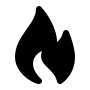
\includegraphics[width=6mm]{images/imageb.png}}; }}

\newtcolorbox{shortcut}{enhanced,arc=0mm,colback=yorhabg,colframe=mred,leftrule=10mm,coltext=yorhafg, coltitle=yorhabg, title=\texttt{Shortcut.}, 
overlay={\node[anchor=west,outer sep=2pt] at (frame.west) {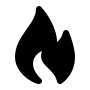
\includegraphics[width=6mm]{images/imageb.png}}; }}

\newtcolorbox{question}{
    enhanced, 
    colback=yorhabg,
    colframe=mblue,
    coltext=yorhafg,
    coltitle=yorhabg,
    attach boxed title to top left={yshift*=-\tcboxedtitleheight}, 
    title=\texttt{Question.},
    boxed title size=title,
    boxed title style={%
        rounded corners=northeast, 
        rounded corners=northwest, 
        colback=tcbcolframe, 
        boxrule=0pt,
    },
    underlay boxed title={%
        \path[fill=tcbcolframe] (title.south west)--(title.south east) 
            to[out=0, in=180] ([xshift=5mm]title.east)--
            (title.center-|frame.east)
            [rounded corners=5pt] |- 
            (frame.north) -| cycle; 
    },
}

\newcommand\bb[1]{\textcolor{yorhafg}{\textbf{#1}}}

\title{\textbf{CSCA67 - Assignment \#1}}
\author{ Satyajit Datta }
\date{\today}

\begin{document}

\maketitle    

\section*{1. Logical Equivalence}
For each of the following pairs of expressions, either prove that the two expressions are equivalent or prove that
they are not. (Clearly state what you are proving!) Do not use truth tables.
\vspace{1em}
\hrule
\vspace{1em}

\begin{question}
    $(a \rightarrow b) \land (b \rightarrow c)$ and $a \rightarrow c$
\end{question}
\begin{center}
        \text{We are proving that the two expressions are not equivalent.} \\
        \text{Consider the case where } a = \text{True}, b = \text{False}, c = \text{True}. \\
\end{center}
\begin{align*}
    & (a \rightarrow b) \land (b \rightarrow c) & & a \rightarrow c\\
    \Rightarrow\; & (T \rightarrow F) \land (F \rightarrow T) & \Rightarrow\; & T \rightarrow T\\
    \Rightarrow\; & F \land T & \Rightarrow\; & \bb{T}\\
    \Rightarrow\; & \bb{F} && \\
\end{align*}
\begin{center}
    $\therefore$ The two expressions are not equivalent. $\blacksquare$
\end{center}

\begin{question}
    $a \land (a \rightarrow b)$ and $a \rightarrow b$
\end{question}
\begin{center}
    \text{We are proving that the two expressions are not equivalent.} \\
    \text{Consider the case where} a = \text{False}, b = \text{True}
\end{center}
\begin{align*}
    & a \land (a \rightarrow b) &  & a \rightarrow b \\
    \Rightarrow\; & F \land (F \rightarrow T)  & \Rightarrow\; & F \rightarrow T\\
    \Rightarrow\; & F \land T & \Rightarrow\; \bb{T} \\
    \Rightarrow\; & \bb{F}
\end{align*}
\begin{center}
    $\therefore$ The two expressions are not equivalent. $\blacksquare$
\end{center}

\begin{question}
    $(a \rightarrow b) \land (a \rightarrow c)$ and $a \rightarrow (b \land c)$
\end{question}
\begin{center}
    \text{We are proving that the two expressions \bb{are} equivalent.}
\end{center}
\begin{align*}
    & (a \rightarrow b) \land (a \rightarrow c) & & a \rightarrow (b \land c) \\
    \Rightarrow\; & (\neg a \lor b) \land (\neg a \lor c) \quad \text{(Conditional Law)} & \Rightarrow\; & \mathbf{\neg a \lor (b \land c)} \quad \text{(Conditional Law)} \\
    \Rightarrow\; & \mathbf{\neg a \lor (b \land c)} \quad \text{(Distributive Law)} & & \\
\end{align*}
\begin{center}
    $\therefore$ The two expressions are equivalent. $\blacksquare$
\end{center}

\begin{question}
    $(a \rightarrow c) \lor (b \rightarrow c)$ and $(a \lor b) \rightarrow c$
\end{question}
\begin{center}
    \text{We are proving that the two expressions \bb{are} equivalent.}
\end{center}
\begin{align*}
    & (a \rightarrow c) \lor (b \rightarrow c) & & (a \lor b) \rightarrow c \\
    \Rightarrow\; & (\neg a \lor c) \land (\neg b \lor c) \quad \text{(Conditional Law)} & \Rightarrow\; & \neg(a \lor b) \lor c \quad \text{(Conditional Law)} \\
    \Rightarrow\; & \mathbf{(\neg a \land \neg b) \lor c} \quad \text{(Distributive Law)} & \Rightarrow\; & \mathbf{(\neg a \land \neg b) \lor c} \quad \text{(De Morgan's Theorem)} \\
\end{align*}
\begin{center}
    $\therefore$ The two expressions are equivalent. $\blacksquare$
\end{center}

\begin{question}
    $a \iff b$ and $(a \land b) \lor (\neg a \land \neg b)$
\end{question}
\begin{align*}
    & a \iff b & & \mathbf{(a \land b) \lor (\neg a \land \neg b)} \\
    \Rightarrow\; & (a \rightarrow b) \land (b \rightarrow a) \quad \text{(Biconditional Law)} \\
    \Rightarrow\; & (\neg a \lor b ) \land (\neg b \lor a) \quad \text{(Conditional Law)} \\
    \Rightarrow\; & (\neg a \land \neg b) \lor (\neg a \land a) \lor (b \land \neg b) \lor (b \land a) \quad \text{(Distributive Law)} \\ 
    \Rightarrow\; & \mathbf{(\neg a \land \neg b) \lor (a \land b)} \quad \text{(Negation Law)}
\end{align*}
\begin{center}
    $\therefore$ The two expressions are equivalent. $\blacksquare$
\end{center}

\begin{question}
    $a \rightarrow (b \rightarrow (c \rightarrow d))$ and $(a \land b \land c) \rightarrow d$
\end{question}
\begin{align*}
    & a \rightarrow (b \rightarrow (c \rightarrow d)) & & \mathbf{(a \land b) \lor (\neg a \land \neg b)} \\
    \Rightarrow\; & \neg a \lor (\neg b \lor (\neg c \lor d)) \quad \text{(Conditional Law)} \\
    \Rightarrow\; & (\neg a \lor \neg b \lor \neg c) \lor d \\
    \Rightarrow\; & \neg(a \land b \land c) \lor d \quad \text{(De Morgan's)} \\
    \Rightarrow\; & \mathbf{(a \land b \land c) \rightarrow d} \quad \text{(Conditional Law)} \\
\end{align*}
\begin{center}
    $\therefore$ The two expressions are equivalent. $\blacksquare$
\end{center}

\begin{question}
    $(a \rightarrow b) \lor (b \rightarrow a)$ and $a \iff b$
\end{question}
\begin{center}
        \text{We are proving that the two expressions are not equivalent.} \\
        \text{Consider the case where } a = \text{True}, b = \text{False}. \\
\end{center}
\begin{align*}
    & (a \rightarrow b) \land (b \rightarrow a) & & a \iff b\\
    \Rightarrow\; & (T \rightarrow F) \lor (F \rightarrow T) & \Rightarrow\; & (a \rightarrow b) \land (b \rightarrow a) \quad \text{(Biconditional Law)}\\
    \Rightarrow\; & F \lor T & \Rightarrow\; &  (T \rightarrow F) \land (F \rightarrow T)\\
    \Rightarrow\; & \mathbf{T} & \Rightarrow\; & F \land T \\
    & &  \Rightarrow\; & \mathbf{F} \\
\end{align*}
\begin{center}
    $\therefore$ The two expressions are not equivalent. $\blacksquare$
\end{center}





\end{document}